%% Benjamin Williams <bwilliams@lincoln.ac.uk>
%% Get in touch if you have any questions or problems!
%% University of Lincoln Computer Science Thesis Template

%% @version     1.0.7
%% @lastchanged 26/04/2021

% The document class -- remove [harvard] if you want
% numeric-style referencing.
\documentclass[harvard]{lincolncsuthesis}
% Packages you want to use
% Packages you intend to use
% ..

% For example, if you want to render 
% the document in a different font you can
% use something like: 

%\usepackage{gentium}
%\usepackage{txfonts}
%\usepackage[sfdefault]{roboto}


% Or maybe you want clickable references in your thesis:
\usepackage{url}
\usepackage{float}
\usepackage{hyperref}
\hypersetup{%
    pdfborder = {0 0 0}
}
\usepackage[UKenglish]{babel}
\usepackage[T1]{fontenc}
\usepackage[utf8]{inputenc}
\usepackage{lmodern}
\usepackage{paralist}
\usepackage{fancyhdr}
\usepackage{amsmath, amssymb, amsfonts}
\usepackage{mathtools}
\usepackage{framed}
\usepackage{pstricks}
\usepackage{graphics}
\usepackage{nomencl}
\makenomenclature
\renewcommand{\nomname}{List of Abbreviations}

\usepackage[amsmath,framed, thmmarks, standard]{ntheorem}
\usepackage[usenames,dvipsnames,svgnames,table]{xcolor}
% \usepackage[backend=bibtex]{biblatex}
% \usepackage[backref=true, hyperref=true, firstinits=true, indexing=true, url=false, style=ieee, backend=biber,  doi=false, texencoding=utf8, bibencoding=utf8]{biblatex}

% Bibliography setup: import bib files
% Add in the .bib files you wish to add 
% into your document here. If you want to
% include others, just copy this line and
% change the path!

\addbibresource{./bib/references.bib}


% This thesis template also supports rendering
% a ludography. To cite games, make sure your reference
% in your bib file has keywords={game} in the bibtex item.
%
% See the bib file below for an example.

% \addbibresource{bib/ludography.bib}

% Your thesis details -- edit the file at the path below
% so it shows your name, title, etc. 
%% Below are a bunch of details for formatting your undergraduate thesis.
%% Make sure to fill each of these out.

% The title of your thesis (If your title is very large, consider prepending
% it with the \Large command
\title{\bfseries Brain-Computer Interface controlled simulated car using CARLA}

% Your name, as an author
\author{Mangal Deep B.M.}

% The degree
\thesisDegree{Master of  Engineering}

% The programme
\thesisProgramme{Embedded Systems for Mechatronics}

% The school name
\thesisSchool{Faculty of Information Technology}

% The university you're studying at (Lincoln!)
% The university (UoL)
\thesisUniversity{Dortmund University of Applied Sciences and Arts}

% Your student number
\thesisStudentNumber{7206937}
\thesisSupervisor{Dr. Andreas Becker}
% The date (which is shown last, you can just put a year in here):

\date{14-March-2023}



% What will be displayed in the header: the assessment item
\thesisHeaderContents{Master Thesis}

% Uncommenting the \thesisTurnOffHF line below will remove your name + id from the footer
% as well as removing the header contents. It is NOT recommended to do this
% as the presentation policy for assessed work in the SoCS requires
% these both of these. However, you may want to uncomment this for other
% reasons: i.e. when printing a personal copy which is NOT going to be
% submitted.
% -----
% \thesisTurnOffHF
% -----
% Not from the University of Lincoln? These commands below might
% be useful to you! Just uncomment them:
% ----------
% \thesisLogoPath{img/your_logo} 
% \thesisProgramme{Biology}
% \thesisSchool{School of Biology}
% \thesisCollege{College of Science}
% \thesisUniversity{Hogwarts School of Witchcraft and Wizardry}
% \thesisSubmissionText{This is some text}
% ----------


% Don't like the table of contents, list of figures, or list
% of tables? Do you want to disable them? If so, uncomment
% the appropriate lines below:
% ---------------
% \turnOffTOF          % List/Table of Figures
% \turnOffTOT          % List/Table of Tables
% \turnOffTOC          % Table of contents
% ---------------



% Do you want to enable listing sections before the thesis
% body in the table of contents? e.g. Abstract, List of Tables,
% List of Figures, etc.
% 
% This is what the command below does.
% 
% Just uncomment it if you this is what you desire:
% -----------------
% \enableManualTOCEntries

% But what if you want to remove "List of Figures", "List of Tables",
% and "Table of Contents" from the table of contents, but leave
% your original sections? That's ok, just uncomment the line below:
% ------------------
% \disableTableTOCEntries

\begin{document}

% First, make the title
\maketitle

% Input anything that can go before the acknowledgements 
%% The blank page environment allows you to insert
% pages into your thesis for specific things

\begin{blankpage}
    \chapterTitle{A blank page}
    This is an optional page environment you could use for things like:
	\begin{itemize}
		\item Your own custom preamble chapters (use \texttt{\textbackslash chapterTitle} for titles!)
		\item \emph{``This work is dedicated to Dad and Mom''}
		\item A copyright notice
		\item Additional notes
		\item Quotes
		\item List of publications
		\item An actual blank page
		\item Nomenclature / glossaries, etc.
	\end{itemize}
	It is not recommended to use this in your undergraduate thesis for submission. It has been left in here to make you aware of its existence. This is largely because it does not follow the guidelines set out for undergraduate theses, but you could include this environment for your own personal printed copy. Consult with your supervisor to see if you can use it. 
	
	In addition, you can pass an optional parameter to this environment with the value \texttt{c} to centre this text vertically on the page (use the \texttt{center} environment to align horizontally).
\end{blankpage}


% Then the abstract
\begin{abstract}
    This is where your abstract will go. Usually this is written last, after writing the entirety of your thesis.
\end{abstract}

% Then the acknowledgements
%\begin{acknowledgements}
Firstly, I want to thank Dad and Mom.\footnote{Here is a footnote} Here is another note.
\end{acknowledgements}

% Print out the table of tables and table of figures and
% tell the template we're about to start the body of the
% thesis.
\thesisTables
% Indexes, Glossaries

\thesisBodyStart
% start of thesis body
% ---------------------------

% Include introduction
\chapter{Introduction}
% \section*{Introduction}
Human computer interaction has been evolving over the past decades. With development in technologies, the physical contact between the computer and the human is decreasing rapidly. Advanced systems which work on speech and gesture control still require a minimal effort from the user to interact with the machine. Though these effort seem to be mere, it is a challenging task for humans with disabilities. Systems which work on facial gestures bridge this gap to an extent but it does not completely decode the actual intent of the person. Brain Computer Interface paves way to encode the persons intent and thoughts without the need for any physical effort. It provides enormous capabilities for physically challenged people to express themselves just by their thoughts. 

Autonomous vehicles are the future of mobility, several companies around the world invest and research on new technologies to solve new challenges that appear in developing level 5 autonomy. The level of human interaction with the vehicle has been decreasing with increasing safety. However including humans in the loop is necessary at certain times to avoid any undesirable events. Level 5 autonomous vehicles is still a long way to go, but by bringing in a minimal interaction of the driver with the system, safety can be improved. One of the ways of achieving it is interfacing the thought and decision process of the driver to the autonomous vehicle, a process commonly referred to as Brain-Computer-Interface (BCI)\nomenclature{BCI}{Brain-Computer-Interface}. 

Once shown in science fiction novels and movies, Brain-Computer Interface (BCI) has become widely researched and developed in the academic institutions and industries in the past decades. It has been applied and tested on mammals for a wide range of applications. However it has its own challenges and limitations. With evolving technologies, new innovations and discoveries, BCI systems are built to understand and decode the brain waves better. The analysis of the brain signals have seen a shift in the paradigm with the introduction of machine learning techniques. 

Modern BCI design involves understanding brain dynamics, pattern recognition in the brain waves, deriving relevant features from the measured brain waves. However it is very challenging to create a BCI system that can work on any person, as the brain signals are task-specific and brain signal signatures are very unique to a person. The cortex folding and the relevant functional maps are different across individuals. Even for the very same person, the brain dynamics are non-stationary at all time scales. In addition, it is almost impossible to place the electrodes exactly on the same location for every recording sessions. Further the psychological states of the user such as boredom, distraction and similar factors play a significant role in the quality of the signal measured. The Signal-to-Noise Ratio (SNR) \nomenclature{SNR}{Signal-to-Noise Ratio} in a brain signal is very poor, making it difficult to obtain required information from brain signals. It is harder to spatially measure the data from one region as large collections of neurons are involved in many different activity, not just one. These challenges can vary a lot depending on the methods used to record and analyse the brain signals as well as the task that needs to be achieved. 

Given the challenges, the goal of this work is to steer a simulated car in the CARLA environment using brain signals obtained from the OpenBCI headgear. CARLA is an open-source simulator to develop, train and validate autonomous driving systems. OpenBCI is an open-source BCI platform that develops hardware and software for BCI scientific research. The brain signal from a 16 channel OpenBCI headgear is fed through a signal processing pipeline to extract the relevant Motor Imagery (MI) \nomenclature{MI}{Motor Imagery}features and classify the users intention. The signal preprocessing pipeline constitutes reliable and conventional signal processing techniques as well as state-of-the-art deep learning techniques. Several tools, libraries and frameworks such as MNE, Numpy, Scipy, Scikit-learn and PyTorch are used to achieve the goal. The communication between the OpenBCI system and the signal processing pipeline is established using Lab Streaming Layer (LSL)\nomenclature{LSL}{Lab Streaming Layer}. The signal processing pipeline classifies the signal into left, right or straight steering command and it is sent to CARLA through Robotic Operating System (ROS 1) framework\nomenclature{ROS 1}{Robotic Operating System-1}. The algorithms are packed into a ROS package which consists of multi-threaded nodes enabling real-time information transfer to CARLA. All the relevant code and references are made available in GitHub\cite{BCI_MotionControl}. Several open-source datasets are used to setup the basic brain signal processing pipeline and later tuned to work with the data obtained form the OpenBCI headgear.

\section{Environment setup}
The specifications of the system used for this project are listed in the table \ref{tb:specs}. The overview of the implemented system is given in the figure \ref{fig:MT_Overall}.

\begin{figure}[H] 
    \begin{center}
    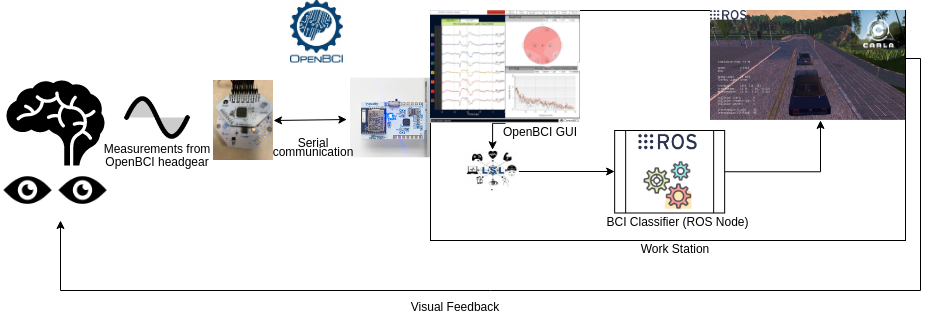
\includegraphics[width=1.0\textwidth]{images/MT_Overall.png}
    \caption{System overview}
    \label{fig:MT_Overall}
\end{center}
\end{figure}

\begin{table}[h!]
\centering
\arrayrulecolor[rgb]{0.8,0.8,0.8}
\begin{tabular}{|l|l|} 
\arrayrulecolor{black}\hline
\multicolumn{2}{|c!{\color{black}\vrule}}{Hardware Specifications}                                                                 \\ 
\hline
Processor                                   & AMD® Ryzen 7 4800h with radeon graphics × 16                                         \\ 
\arrayrulecolor[rgb]{0.8,0.8,0.8}\hline
RAM                                         & 16GB                                                                                 \\ 
\hline
Operating System                            & Ubuntu 20.04.5 LTS 64-bit                                                            \\ 
\hline
\# CPU cores                                & 8                                                                                    \\ 
\hline
GPU                                         & NVIDIA GeForce RTX 2060/ \\ 
                                            & RENOIR (renoir, LLVM 14.0.5, DRM 3.42, 5.15.0-56-generic)  \\ 
\hline
Graphic Card Driver                         & 515.86.01                                                                            \\ 
\hline
CUDA                                        & 11.6                                                                                 \\ 
\hline
cuDNN                                       & 8.3.2                                                                                \\ 
\hline
Cython + Daisy                              & 3.0.0                                                                                \\ 
\hline\\
\hline
%\multicolumn{1}{|l!{\color{black}\vrule}}{} & \multicolumn{1}{l!{\color{black}\vrule}}{}                                           \\ 
\arrayrulecolor{black}\hline
\multicolumn{2}{|c!{\color{black}\vrule}}{Software Specifications}                                                                 \\ 
\hline
Visual Studio Code                          & 1.74.0                                                                               \\ 
\arrayrulecolor[rgb]{0.8,0.8,0.8}\hline
OpenGUI                                     & 5.1.0                                                                                \\ 
\hline
CARLA                                       & 0.9.11 (py3.7-linux-x86\_64)                                                         \\ 
\hline\\
\hline
%\multicolumn{1}{|l!{\color{black}\vrule}}{} & \multicolumn{1}{l!{\color{black}\vrule}}{}                                           \\ 
\arrayrulecolor{black}\hline
\multicolumn{2}{|c!{\color{black}\vrule}}{Libraries and Frameworks}                                                                \\ 
\hline
Numpy                                       & 1.22.3                                                                               \\ 
\arrayrulecolor[rgb]{0.8,0.8,0.8}\hline
Pytorch                                     & 1.12.0+cu116                                                                         \\ 
\hline
MNE                                         & 1.2.0                                                                                \\ 
\hline
OpenCV                                      & 3.4.15                                                                               \\ 
\hline
scipy                                       & 1.8.1                                                                                \\ 
\hline
sklearn                                     & 1.1.1                                                                                \\ 
\hline
matplotlib                                  & 3.4.2                                                                                \\ 
\hline
kymatio                                     & 0.2.1                                                                                \\ 
\hline
PIL                                         & 7.0.0                                                                                \\ 
\hline
pandas                                      & 1.1.4                                                                                \\ 
\hline
Optuna                                      & 3.0.0                                                                                \\
\hline
\end{tabular}
\caption{\label{tb:specs} System and software specifications used for this project.}
\arrayrulecolor{black}
\end{table}

\section{Outline} 
The thesis is organized as follows the chapter \ref{ch:background} provides insight on different brain signal recording techniques, various EEG paradigms, brain signal extraction methods, artifact removal techniques used in this work and brief description of feature extraction, selection and classification steps, \ref{ch:sp_bci} discusses on various feature extraction and classification techniques used in brain signal analysis, \ref{ch:DL_bci} discusses on different SOTA Deep Learning techniques used in BCI signal analysis that can work as feature extractor and classifier. In chapter \ref{ch:cmp_bnch}, the tools and libraries used in this work are explained. The implemented algorithms are compared and analysed for different combinations. Finally chapter \ref{ch:ch_cncl} discusses about the challenges faced, further enhancements and the systems applicability for different use cases.

The following chapters provide deeper intuition and understanding of the methods researched and used in accomplishing this work. Finally the chosen algorithm is used to steer the simulated car in CARLA through ROS.

% Literature review / Background / Related work
\chapter{Literature review}
%%%%%%%%%%%%%%%%%%%%%%%%%%%%%%%%%%%%%%%%%%%%%%%%%%%%%%%%%%%%%%%%%%%%%%%%%%%%%%%%%%%%%%%%%%%%%%%
% Another cool thing about \LaTeX~is its referencing system. This template is set up to use harvard-style referencing. You can do this by using \texttt{\textbackslash citep\{citekey\}}. It will print out something like this: \citep{aad2012observation}. Or alternatively, you can use \texttt{\textbackslash cite\{citekey\}} to cite things like this: \cite{chatrchyan2012observation}. This template uses Bib\LaTeX~for referencing, with a Biber backend. This is primarily due to the extensive features Bib\LaTeX~provides, along with the option of glossaries. If you want to customise the referencing style, you can either modify the template slightly to use different options, or use \texttt{\textbackslash usepackage} again to reimport it. There's probably some commands to change its options after its been imported too.

% \section{Ludography}
% This thesis template also contains an optional ludography. This is primarily for Games Development students, who wish to cite games in their thesis. To use this, just put references into your bib file as usual with the game's details. Then, make sure \texttt{keywords} is set to \texttt{\{game\}}. This is what is used to determine which references are games, and which are actual papers. For a more elaborate example, see \texttt{bib/ludography.bib}.

% Also, make sure that the \texttt{title} key is actually the author of the game, and the \texttt{author} is the title of the game. The reason this is swapped around is because Bib\LaTeX~likes to print references out with the author first. Then, just add \texttt{\textbackslash printLudography} with an optional title argument to print out all citations like \texttt{\textbackslash printLudography} or \texttt{\textbackslash printLudography[Games]}.

% You can also use the \texttt{ludography} environment if you wish to print out some text before the list of games is printed. An example of this can be seen in \texttt{main.tex}. To cite games, you can \texttt{\textbackslash cite} it like any other reference. However, if you want it to display the title instead of the standard referencing style, you can use \texttt{\textbackslash citeGame} instead.

% Here is an example of a cited game with a normal reference style: ~\cite{spaceinvaders}. Ugh, pretty ugly. Instead, here the two are  cited in the next sentence as games with \texttt{\textbackslash citeGame}. Both \citeGame{spaceinvaders} and \citeGame{breakout} were games made by Atari. Much better!

% SLAM Formulation + State Prediction and correction
\chapter{Formulation}
\section*{Introduction}
    The goal of this work is to control the simulated car in CARLA using motor intent from the users brain activity. Motor Imagery is the information that needs to be extracted from the EEG data. There are several other information that can be  obtained and are broadly classified into Spontaneous EEG and Evoked Potential which are briefly explained.

\section{Brain Signal Acquisition/ Extraction}
Neurons are the basic computational unit of the nervous system. The electric signal recorder as brain wave is the result of electrochemical interations that occur at the outer membrane of neurons. In case of a event, the raises and falls of potential at the membrane of the neuron is called as action potential. The electrical activity at the neurons enable us to record and decode the brain activities. There are many ways to record the electrical activity and are broadly classified into invasive and non-invasive recording. Some technologies can also be used to stimulate neurons or brain regions, that allows BCIs to send feedback to brain based on interactions with the world. This work is only on Electroencephalography, a  noninvasive approach, hence the topic on invasive approaches and other noninvasive approaches are just briefly touched.

    \subsection{Invasive Approaches}
Approaches requiring some surgery where an electrode is placed in direct contact with required region in the brain are invasive methods of recording brain signals. These approaches are typically performed on animals such as monkeys, rats. In case of humans these approaches are carried on under strict clinical settings. As the recording sensor is in direct contact with the brain tissues, these provide higher quality signals with high SNR, higher spatial resolution and less spatial smearing compared to the noninvasive approaches.

    \subsubsection{Electrocorticography (ECoG)}
    ECoG is an extracortical invasive electrophysiological monitoring method \cite{2021}. Typically performed in a clinical setting, a strip of electrodes are placed on the surface of intrest on the brain. It has many advantages compared to other invasive approaches.

    \subsection{Noninvasive Approaches}
Approaches that gather brain signals over the surface of the scalp, without any surgery or electrodes being inserted into the skull are termed noninvasive approaches. The signals could be collected by measuring the electrical or the magnetic activity on the surface of the scalp. Some of the common noninvasive approaches are Electroencephalography (EEG), functional magnetic resonance imaging (fMRI), functional near-infrared spectroscopy (fNIRS), magnetoencephalography (MEG), and electrooculography (EOG).
    
%     \subsubsection{Functional Near-infrared Spectroscopy (fNIRS)}
% fNIRS uses near-infrared light to measure the degree of oxygenated and deoxygenated haemoglobin. The relative levels 

    \subsubsection{Electroencephalography (EEG)}
EEG is the most commonly used noninvasive approach used to measure brain electrical activity on the surface of the scalp. The electrodes are usually placed according to internationally recognized 10-20 system \cite{}. The spatial resolution of the signals depend on the number of electrodes used. The temporal resolution depends on how many samples the system could measure in a second. However the temporal resolution of the EEG signals is much better than the spatial resolution. In Comparison to invasive approaches, the EEG systems have poor spatial and temporal resolution, and very poor SNR. Since the measurement is taken
over the surface of the scalp, the obstruction of the skull and other tisses between cortex and the scalp act as a huge conductive surface leading to spatial smearing. In comparison to other noninvasive approaches EEGs have higher temporal resolution, tolerant to noise and artifacts, low cost and no exposure to high intensity magnetic fields.

    Spatial smearing is the effect by which all the electrodes tend to measure the same signal because of the conductive effect of the tissues between the cortex and scalp. It also very succeptible to other noises such as power-line, changind electrode impedance, eye movements, eye blinks, facial muscle movements and head movement. The brain signals measured from the EEG systems can be seperated into frequency bands, where each frequency band represents to a specific brain state
and level of awareness. The recorded brain signals contains information on various physiological, psychological, mental, sensory and cognitive activities. Hence it is required to analyse and extract the relevant information from the signal.

\section{EEG Paradigms}

\subsection{Spontaneous EEG}
Spontaneous EEG also referred as Oscillatory Activity includes a wide range of task typically without any external stimulation such as mental task, motor imagery,sleeping, under fatigue stage. BCI systems that work with spontaneous EEGs are also called Active BCI as they reuire conciously controlled thought independent from external events.BCI systems that work with spontaneous EEG are hard to train given their low SNR and variation in subjects.

    \subsubsection{Motor Imagery (MI)}
Imagining a motor movement without performing an actual movement is termed Motor Imagery. It is one of the widely researched EEG paradigm that is used in several applications where the user is limited in their motor movement capabilities. It also helps in mental rehersals as the person experience themselves performing the action. MI is due to two basic phenomena that occur in the brain onset of imagination - Event Related Desynchronization (ERD) and Event Related Synchronization (ERS). ERD/ERS refers to 
phenomena that the magnitude and the frequency distribution of the EEG signal power changes during a specific brain state. It is mostly observed in sensory, cognitive and motor tasks. During motor imagery contralateral ERD is observed in the mu band and after motor imagery ERS is observed in beta band.

Event Related Desynchronization (ERD) is due to activity of small set of neurons. A visual stimulation results in a short lasting attenuation or blocking of rhythm in the alpha band leading to power decrease of ongoing EEG signals. This decrease in the oscillatory is related to internally or externally paced events.

Event Related Synchronization (ERS) is due to activity of large set of neurons. The increase in oscillatory activity is again related to internally or externally paced events.It is characterized by short lasting amplitude enchancement.

\subsection{Evoked Potential (EP)}
Processing of physcal stimulus rather than higher processes that might involve memory and attention. BCI systems that work with EPs could be also called Reactive BCI as they rely on response to the stimulus provided. Few of the commonly researched EPs are described below.

    \subsubsection{Event Related Potential (ERP)}
It is the most widely researched EPs and it is further classified based on the stimulus used to trigger the brain waves: visual evoked potential when stimulated visually, audiotory evoked potential when stimulated with sound and somatosensory evoked potential when evoked with smell. The stimulus could be internal or external based on the BCI system. P300 is an important component in ERP and it is been widely used in many BCI systems exiisting in the marker. It refer to the postive peak that appears 300ms after the onset of stimulus.

    \subsubsection{Error Related Potential (ErRP)}
It is a result oof an errorous event. It is generated by the error processing mechanism in the human brain. It provides a feature rich feedback to the BCI system and helps to tune the sytem in the desirable way.

\section{Brain Signal Processing Pipeline}
The brain signal is fed through several signal processing algorithms to extract the best possible information. These processing algorithms are specifically chosen to  extract motor imagery data. The overall processing pipeline is given in the figure \ref{}. THe first few steps in the processing pipeline is the same for both conventional and deep learning approaches.  The variation is observed only at feature extraction and classification. These steps involved in the pipeline are explained in detail in the following sections.

\subsection{Data Extraction}
The input to the pipeline could be an online/offline data from OpenBCI headgear or publicly available open-source datasets. The open-source datasets were used in order to design the pipeline and later the pipeline is calibrated to work with data from OpenBCI headgear.

\subsubsection{OpenBCI headgear}
Before the experiment could be started several parameters are checked. In order to ensure the contact of electrodes on the users scalp, the impedance at the electrodes are monitored and adjusted untill they fall into acceptable threshold i.e. less than $750K\Omega$. Next the frequency filters are configured to avoid DC offset and electric powerline noises. However this filter is applied only to the visualizer and not to the recorded data. The electrodes are very succeptible to noises that appear around 25Hz even after
filtering the DC offset and powerline noises. Hence while performing the experiment the user is away from any electronic device.

Establihing a proper experiment is a key step in training the classifiers, By \cite{} each trail is recorded for 12 seconds, the setup used to gather data for a three class system that consists of a window sperated by a vertical line and two squares - yellow and blue,  in the centre initially. The beginning of each trial is marked by change in color of the vertical line then the subject is requested to be in a idle state for the first 5 seconds. The motor imagery task to be performed is presented on the screen  for 3 seconds with help of a yellow square by moving it to the left,right or standstill denoting only straight motion without steering, here the subject can prepare themselves. After which the subject either performs the instructed movement or imagines performing the movement for 3 seconds. The data collected so far could be wither used to train a model online or it can used as input to a presaved model and obtain the classification result. The result of the classifier is used to move the blue square accordingly. The answer presented to the subject stimulates feedback in the user which is again captured in the recording for analyzing ErRP and to improve the classifier results.

LSL is used to establish communication between OpenBCI GUI and CARLA BCI Control ROS node. With the support of MNE, a mock LSL stream can be used to stream recorded data which helps in debugging the algorithm even in the absence of the OpenBCI headgear.

\subsubsection{Open-source Datasets}
    BCIs are widely researched topic for several decades, however the huge variation in the BCI experiments to obtain relevant information from the brain signal is a bottleneck in the publicly available dataset. This work required a multiclass motor-imagery dataset recorded with 16+ channel BCI system and sampling rate of greater than 125Hz. Some of the datasets that were used in setting up the signal processing pipeline and used for comparative analysis are discussed further. The dataset thus used were resampled, channel picked inorder to develop a signal processing pipeline compatible to the hardware inhand.

\subsubsection{PhysioNet}
    It consists of over 1500 one- and two-minute EEG recordings from 109 participants performing motor-imagery task using 64-channel BCI2000 system at a sample rate of 160Hz. Each participants performed 14 experiments each involving either imagining or actually performing opening and closing fists and feet. The BCI system followed the international 10-20 system making it easy to construct MNE Raw frame.

\subsubsection{Berlin BCI Competition}
    This compettion was held for few years where the competitors had to come up with the best performing signal processing pipeline for dataset. This includes a list of various EEG datasets, this work uses the motor imagery dataset from BBCI III IVa. The recordings were performed using 118-channel EEG system at a sampling rate of 1000Hz. It consists of 5 participants, each performing motor imaginaton of right fist or foot. The electrode locations in the BCI system is arbitrary and the location info was provided with the dataset. It required manual asssignment of locations to enable all the functionalities in MNE framework. From this point the word- dataset and data are used interchangibly and it is used to denote the data obtained from the OpenBCI headgear and the open-source datasets unless specified.

\section{Preprocessing}
The data obtained needs to be processed effectively to get the best possible information and it influences the classification result dramatically. Most of the BCI systems in the literature use the following techniques to achieve the best results. 

\subsection{Artifact removal techniques}
    Any undesirable signals that originate outside the brain  are termed artifacts. Some of the artifacts are listed in the section. Techniques that are used to remove such artifacts from relevant data are effective on one such artifact. Techniques described below are proved to be effective for this work. 

\subsubsection{Band Pass}
The information required to perform motor imagery classification is present in the low frequency region i.e 30Hz, hence bandpassing the signal between 5Hz and 40Hz removes the DC offset and irrelavant information. It also avoids the need for a notch filter at 50Hz or 60Hz to remove the electric power line noise. 

\subsubsection{Spatial Filtering}
The potential that is measured at an electrode is overlap or a linear combination of several sources in the brain, this is primarily due to volume conduction. Given $\mathcal{x}_i$ from n independent sources, the sum of all independent sources can be written as \ref{eq:spat_smear}.

\begin{equation} \label{eq:spat_smear}
    \mathbb{C}^{j} = \sum_{n = i}^{n} w_{i}^{j} x_{i} = \mathbb{W^{j} X} 
\end{equation}

where $\mathbb{C}^{j} $ refers to measurement from arbitary channel $j$,  $\mathbb{W^j}$ represents the weight matrix for channel $j$ and $\mathbb{X}$ represents independent sources. Inherently brain signals are low in SNR, improving the SNR would enable increased classification accuracy. Spatial filtering achieves this by performing one of the following - enhance local activity, reduce noise across channels, dimensionality reduction, identify hidden sources, find projections that maximize discrimination between different classes. The following techniques perform one of the above mentioned operations. Spatial Filters also help to invert measurement to the
original source.

\subsubsection{Bipolar Referencing}
Rereferencing the measurement from the electrodes is one of the common methods that help to achieve better SNR.

For a primitive system, Bipolar rereferencing will highlight the required features by finding the potential difference between two electrodes of interests. Consider measurement from channels $i$ and $j$

\begin{equation} \label{eq:bip_eeg}
    \mathbb{C}^{i}_{Bi} =  \mathbb{C}^{i} - \mathbb{C}^{j}
\end{equation}

\subsubsection{Laplacian Referencing}
Laplacian rereferencing enhances local activity at the electrode of interest by subtracting the potential of the channel of interest from the potentials of the adjacent four channels $\theta$. This is achieved by removing the muscle activity from the electrode of interest.

\begin{equation} \label{eq:lap_eeg}
    \mathbb{C}^{i}_{LP} =  \mathbb{C}^{i} - \frac{1}{4} \sum_{i \epsilon \theta} \mathbb{C}^{i}
\end{equation}

\subsubsection{Common Average Referencing (CAR)}
It is the most common method of rereferencing, it is very similar to Laplacian rereferencing, but instead of the adjacent electrodes, the average of potentials of all the electrodes is subtracted.

\begin{equation} \label{eq:car_eeg}
    \mathbb{C}^{i}_{CAR} =  \mathbb{C}^{i} - \frac{1}{N} \sum_{n = 1}^{N} \mathbb{C}^{i}
\end{equation}

\subsubsection{Independent Component Analysis (ICA)}
The potentials recorded using EEG electrodes appear the same and it is highly corelated. This measurement is highly redundant as it doesn't provide any distinctive features that could enable efficient classficiation. Principal Component Analysis (PCA) enables dimensionality reduction that helps to remove the redundant information by finding the dimensions of highest variance , also called as principal components and transforming the measured data to the directions of N desired principal components that contains the most valuable information. With reduced dimensionality the classifier can be trained effectively as the principal components serve as feature vectors as they have the necessary information. Though the transformed data is decorrelated, the higher orders of the data are not independent, i.e. the transformed data is not completely independent. For analysis of brain signals, the measured data is assumend to be a linear combination of statistically independent signals from different regions in the brain, hence complete independence of the data is essential.

Consider $\mathbb{X}$ independent sources, the measurement $\mathbb{C}$ at the channels is mixed up by mixing matrix $\mathbb{M}$ \ref{mixed_ica}.

\begin{equation} \label{eq:mixed_ica}
    \mathbb{C} = \mathbb{MX} 
\end{equation}

ICA helps to recover the independent sources by finding the unmixing matrix  $\mathbb{M^{-1}}$ \ref{unmixed_ica} in case where the n independent sources and N channels are the same.

\begin{equation} \label{eq:unmixed_ica}
    \mathbb{X} = \mathbb{M^{-1}C}
\end{equation}

However the independent sources $\mathbb{X}$ obtained from ICA can be less than, more than or equal to the number of measured channels and not orthogonal to each other unlike PCA. These independent components serve as feature vector for classification or removes the artifacts from the measurement.

\subsubsection{Signal Space Projection (SSP)}
It helps in removing the artifacts in the signal by estimating a projection matrix based on measurements with and without signals of interest. The measurements are first taken without a subject to determine the directions of the noise vectors and the matrix formed by the noise vectors is used to project the measurement onto the hyperplane orthogonal to the noise vectors to remove the noise from the measurement data. Noise reduction leads to loss of dimensions however it is relatively less compared to original signal space.  

\section{Epoching}
After preprocessing the measurement, the data that is stored in the RAW format cannot be used further for feature extraction or classification as it conssits of information relating to all the classes, hence the data has to be broken down into segments with a specific time bound before and after the event, grouped together based on the class. This process is referred to as epoching. This enables extraction of distinctive features that is most prevalant in all the segments in a particular class. The data after epoching is of the shape $Ep \times N \times T$. where  $Ep$ is the nummber of epochs that is equal to the number of events, $N$ channels and $T$ epoched time points which is roughly between
$-8$ and $4$ with the event trigger at the $0$ mark.

The frequency spectra of brain signals commonly have the $\frac{1}{f}$ structure, where the low frequency components domainate the results of the analysis. Power normalization resolves this by removing the $\frac{1}{f}$ and it is performed with the help of baselining the segments. Baseline is defined as a time intreval usually before the occurence of the event.

Power normalization is the ratio of activity (TF power) to baseline (TF power for a specific time window) \ref*{bel}.
\begin{equation} \label{eq:bell}
    10\log_{10}(\frac{activity}{baseline})
\end{equation}

Apart from power normalization, baselining helps in seperating task from background activity, normally distributes the data and makes it easier to compare the values across individuals and frequencies.

\section*{Summary}
From here the clean data is fed to conventional approaches and deep learning approaches seperately.

\chapter{Particle Filter}
\section*{Introduction}
Parametric filters such as EKF work on the assumption that posterior density is Gaussian parameterized by mean and covariance. In cases where the true density is non Gaussian, these filters fail to describe the actual posterior. In many practical applications, linear and Gaussian assumptions would not hold true, hence better approaches are required to describe the posterior density. Particle Filters are non parametric filters which can model any posterior distribution as it does not assume to be Gaussian. This chapter provides in-depth view of particle filters and its application to SLAM.
%%%%%%%%%%%%%%%%%%%%%%%%%%%%%%%%%%%%%%%%%%%%%%%%%%%%%%%%%%%%%%%%%%%%%%%%%%%%%%%%%%%%%%%%%%%%%%%%%%%%%%%%%%%%%%
\section{Particle Filter}
Particle Filters manage to model the required distribution by use of a set of random samples sampled from the distribution. However no a-prior information about the distribution is known. Hence a proposal distribution is used as a initial guess to sample particles from it and weigh it against the target distribution. This process is repeated until the proposal distribution matches the target distribution and it requires re-sampling from the proposal distribution when necessary. The samples which weigh more are more likely to describe the target distribution. This leads to further discussion on what could be the guess on proposal distribution, how is it sampled, weighed, re-sampled and sequentially continued to obtain the full state estimate.

\subsection{Sample}
Sampling in particle filters in based on Sequential Importance Sampling principle and Sequential Monte-Carlo methods. Samples in general are generated in random from a proposal distribution. The more samples we are able to sample , the better is the approximation of the target distribution. With larger number of samples, Monte-Carlo methods provide equivalent representation of the target distribution and Sequential Importance Sampling approaches optimal Bayes estimate \cite{S.Arulampalam}. In case of the Monte-Carlo approximation methods, the samples obtained are independent samples of the target distribution, whereas in the Importance Sampling method, the samples obtained are not only independent of the target distribution but independent on the proposal distribution as well. Thus the weights of each sample are not equal as in the case of Monte-Carlo approximation methods.

Let ${x^{1},x^{2},.........x^{N}}$ be list of ${N}$ particles generated from the proposal distribution ${q(x)}$.

\begin{gather} \label{Sample}
    p(x) \approx \sum_{i = 1}^{N} w^{i}\delta (x - x^{i})  
\end{gather} 
where $\delta$ is the impulse function. The above equation provides the weighted approximation of the true density given that the proposal distribution is similar to the target distribution and it is easy to sample from the proposal distribution. A typical example of a proposal distribution is Gaussian. However modeling the proposal distribution effectively for the task is discussed in later sections.

\subsection{Importance weighting}
Importance weighting is an useful outcome of Importance sampling. Each particle is weighed based on its similarity to the target distribution. More the similarity higher is the value of the weights. 
\begin{gather} \label{ImportanceWeigting}
    w \propto \frac{p(x)}{q(x)} 
\end{gather}
The weights are always normalized for reasons discussed further below.

\subsection{Sequential Importance Sampling}
Sampling and weighting discussed above are useful to estimate the state for a given instance. However in most applications it is required to estimate the state recursively for every time instance using the previous state and the current reading. This is the core of the Sequential Importance Sampling. It involves sampling,weighting recursively. In the sampling step as the the sample from the motion model estimate is sufficient as the prior information until the previous instance is already processed.
For the ${i}^{th}$ particle:
\begin{gather} \label{SIS_Sample}
    x_{0:t}^{i} \approx q(x_{0:t}| y_{1:t}) 
\end{gather}
where ${q(x_{0:t}| y_{1:t})}$ is the posterior density of the proposal distribution which could be factorized as 
\begin{gather} \label{SIS_propfact}
    q(x_{0:t}| y_{1:t}) = q(x_t|x_{t-1},y_{t}) q(x_{0:t-1}| y_{1:t-1}) 
\end{gather}
In the weighting step the proposal is compared to the target density also considering its prior weight update. 
\begin{gather} \label{SIS_weight}
    w_{t}^{i} = w_{t-1}^{i} \frac{p(y_{t}|x_{t}^{i}) p(x_{t}^{i}|x_{t-1}^{i})}{q(x_t|x_{t-1},y_{t})}  
\end{gather}
With the right choice of the proposal distribution the weights can be derived with measurement model.
\begin{gather} \label{SIS_weightprop}
    q(x_t|x_{t-1},y_{t}) = p(x_t|x_{t-1})\\
    w_{t}^{i} = w_{t-1}^{i} * p(y_{t}|x_{t}^{i})
\end{gather}
In most cases the weights of the particles in a sample set can end up with high variance, due to which the particle with the highest weight gets sampled repeatedly in the re-sampling step. This is referred to as Particle Degeneration. Hence the system's belief is stuck to one particle leading to ignorance of uncertainty and consecutively to divergence of the filter from the true value.

\subsection{Resample}
As the variance of the weights increase the sample set is dominated only by very few particles with high weight which results in poor state estimate. Hence to avoid it is better to perform a re-sampling step where N particles are sampled from the current particle set using various strategies. Depending on the strategies used to re-sample various re-sampling techniques exists such as Systematic re-sampling, Random re-sampling, Selective re-sampling \dots. This replaces the old sample set with new set of samples with equal weights. However in most cases the clarity of tolerable variance of the weights for a particle set is not clear. It is found that Adaptive re-sampling provides the best criteria for re-sampling. This requires calculating the effective number of the particles ${N_{eff}}$
\begin{gather} \label{Neff}
N_{eff} = \frac{1}{\sum_{i=1}^{N} w_{i}^{2} } 
\end{gather}
where ${w_{i}}$ is normalized weight of the particles in the sample set and ${N}$ is the number of particles.  Re-sampling is performed only 
when the ${N_{eff} < N/2}$.
%%%%%%%%%%%%%%%%%%%%%%%%%%%%%%%%%%%%%%%%%%%%%%%%%%%%%%%%%%%%%%%%%%%%%%%%%%%%%%%%%%%%%%%%%%%%%%%%%%%%%%%%%%%%%%
\section{Rao-Blackwellized Particle Filter}
 This method exploits the spatial structure in particle filter. Instead of applying particle filter on all dimensions, use particle filter only in few dimensions but exploits linearity in other dimensions. In case of SLAM the joint posterior $p(x_{1:t}, m | z_{1:t}, u_{1:t-1})$ can be factorized as 
\begin{gather} \label{RAoB}
    p(x_{1:t}, m | z_{1:t}, u_{1:t-1}) = p(m | z_{1:t}, x_{1:t}).p(x_{1:t} | z_{1:t}, u_{1:t-1})
\end{gather}
where the problem of solving the joint posterior disintegrates to $p(m | z_{1:t}, x_{1:t})$ mapping which is the linear part in the spatial structure and $p(x_{1:t} | z_{1:t}, u_{1:t-1})$ localization where particle filter can be applied. By estimating the trajectory of positions, then the mapping can be performed easily. With the right choice of the proposal distribution, where it can be resolved into recursive terms as in \refeq{SIS_propfact} then the weight calculation can also be done recursively.
\begin{gather} \label{RaoB_weight}
    w_{t}^{i} = w_{t-1}^{i} \frac{p(z_{t}|x_{t}^{i}, m_{t-1}^{i}). p(x_{t}^{i}|x_{t-1}^{i}, u_{t-1})}{q(x_t|x_{t-1}^{i},z_{t}, u_{t-1})}
\end{gather}
This is followed by the re-sampling step and the estimation is carried over recursively.
%%%%%%%%%%%%%%%%%%%%%%%%%%%%%%%%%%%%%%%%%%%%%%%%%%%%%%%%%%%%%%%%%%%%%%%%%%%%%%%%%%%%%%%%%%%%%%%%%%%%%%%%%%%%%%
\section{gMapping-Improved RBPF}
The proposal distribution discussed so far use the motion model which is easy to compute for most type of robots and recursive calculation of the importance weights used only the measurement model to update the previous importance weight. However this can result in sub-optimal results as a laser sensor could provide better accurate information than the motion estimate. Hence using the sensor observation in the proposal distribution can provide better approximation than the motion estimate. In the case of grid mapping the number of occupied cell state explodes which makes it difficult to calculate the importance weight update recursively. Hence the known proposal distribution can be obtained using the adapted particle filter where the proposal distribution of each particle is derived from sampled estimate of optimal proposal distribution. It is observed that the likelihood of the robot position with the help of sensor observations has only one peak with small variance. Hence limiting the sample of the proposal to this likelihood would help in reduced sample set as very few particles can easily describe the distribution. 
\begin{gather} \label{gMap-L}
    L^{(i)} = \{ x | p(z_t| m_{t-1}^{(i)},x)>\epsilon\} 
\end{gather}
This region consists of information from the observation likelihood and motion model. In order to determine the region of maximum likelihood a scan matching procedure is applied. 
\begin{gather} \label{gMap-SM}
    \hat{x_t} = argmax_x p(x|m_{t-1}^{(i)}, z_t, x_t^{(i)})
\end{gather}
Several scan matching procedures are experimented in this thesis and it will be described and compared in the later chapters. With the region of high likelihood derived now a second generation of samples are generated 
\begin{gather} \label{gMap-2samp}
    x_k \approx \{x_j | |x_j - \hat{x^{(i)}}|<\epsilon \}
\end{gather}
can be efficiently derived from which mean and variance of the sample set is calculated. 
\begin{gather} \label{gMap-mu}
    \mu_t^{(i)} = \frac{1}{\eta}. \sum_{j = 1}^{k}  x_j.p(z_t | m_{t-1}, x_j). p(x_j | x_{t-1}, u_{t-1}) \\
    \varSigma_t = \frac{1}{\eta}. \sum_{j = 1}^{k}  p(z_t | m_{t-1}, x_j). p(x_j | x_{t-1}, u_{t-1}).(x_j - \mu_t).(x_j - \mu_t)^T \\
    \eta = \sum_{j = 1}^{k}  p(z_t | m_{t-1}, x_j). p(x_j | x_{t-1}, u_{t-1})
\end{gather}
This leads to the efficient recursive calculation of the importance weights.
\begin{gather} \label{gMap-w}
    w_{t}^{i} = w_{t-1}^{i}.\eta
\end{gather}
However in situations in which the scan matching fails, motion model estimate is used to estimate the most likely position and derive the second generation samples.
\begin{gather} \label{gMap-MM}
    \hat{x_t} = p(x|m_{t-1}^{(i)}, z_t, x_t^{(i)}) \\
    w_{t}^{i} = w_{t-1}^{i}.p(z_t | m_{t-1}, x_j)
\end{gather}
Finally when the variance of the weights increases as per the Adaptive Re-sampling criteria discussed earlier, then Re-sampling can be carried out on the existing particle set.

%%%%%%%%%%%%%%%%%%%%%%%%%%%%%%%%%%%%%%%%%%%%%%%%%%%%%%%%%%%%%%%%%%%%%%%%%%%%%%%%%%%%%%%%%%%%%%%%%%%%%%%%%%%%%%
\section{Results and Analysis}

%%%%%%%%%%%%%%%%%%%%%%%%%%%%%%%%%%%%%%%%%%%%%%%%%%%%%%%%%%%%%%%%%%%%%%%%%%%%%%%%%%%%%%%%%%%%%%%%%%%%%%%%%%%%%%
\section{Summary}

\chapter{Scan Matching}
\section*{Introduction}
Unveiling the full potential of LiDAR and its robustness in creating a scan map of the environment,
LiDAR Odometry and Mapping(LOAM) was presented in \cite{ZhangS14}. In this approach only a subset of the point clouds is used to extract useful features such as planes, lines and edges which is later 
used to derive various metrics for the scan registration. In \cite{D.Hahnel}, consistent Maps were generated with the help of 2D scan matching and also were able to detect and track people
even with the help of sample based Joint Probabilistic Data association filter.
Depending on how the point cloud data is modelled existing approaches can be classified into 
global and local scan matching. In global scan matching the point cloud is considered as a whole, but in local scan matching only segments of the point cloud are matched.

Some of the local scan matching approaches include Iterative Closest Point(ICP), Normal  Distribution Transform(NDT) and Global scan matching approaches include Correlative Scan Matching(CSM)

\section{Iterative Closest Point}
It is the most well-known widely used algorithm known for  efficient registration of given two 2D or 3D scan or point cloud data under euclidean transformation. It is the most simple and intuitive algorithm. Provided the correspondence between the points in the point cloud and with a  approximate initial guess, ICP tries to find the optimal motion parameters - rotation $\mathcal{R}$ and translation $\mathcal{T}$ of given two point cloud data. In practice the correspondence is usually unknown, hence iterative procedure is followed with good initial guess. If the initial guesses are close enough ,a converging solution is obtained. The iteration is generally stopped after certain number of iterations or if the error value reaches below a threshold. Different variants of ICP are developed such as Point-to-Point, Point-to-Plane, Plane-to-Plane each with its pros and cons. 

\paragraph{ICP using Spectral Value Decomposition}
First proposed in \cite{KS.Arun}, the centroid of the two point cloud data are aligned and relative rotation of the two point cloud data is obtained using SVD such that the least squared error is minimized. In simple words the squared error in the observation from two different relatively close view points need to be minimized. This approach results in closed form solution only when the point correspondence of two point clouds is known. Hence it is iterated over until convergence.
\par
Given the two point cloud data $p_1$ and $p_2$, where $p_2 = \mathcal{R} p_1 + \mathcal{T} + N$, find $\mathcal{R}$ and $\mathcal{T}$ such that error function
\begin{gather} \label{ICP-error}
    E(\mathcal{R}, \mathcal{T}) = \frac{1}{N_{p_1}}  \Sigma_{i=1}^{N_{p_1}}\left\lVert p_2 - \mathcal{R} p_1 -\mathcal{T} \right\rVert^2 
\end{gather}
is minimized.
where $N_{p_1}$ is the number of points in the point cloud data.

It can be accomplished by taking the  of the point clouds $p_{1}$ and $p_{2}$ such that
\begin{gather} \label{ICP}
            \mu_{p_1} = \frac{1}{N_{p_1}} \sum\limits_{i=1}^{N_{p_1}} p_{1_i}\\
            \mu_{p_2} = \frac{1}{N_{p_2}}  \sum\limits_{i=1}^{N_{p_2}} p_{2_i}\\
            P_{1} = p_{1} - \mu_{p_{1}}\\
            P_{2} = p_{2} - \mu_{p_{2}}\\
            H  \triangleq  \sum\limits_{i=1}^{N} P_{1} P_{2}^{T}
\end{gather}
Now to find the rotational component of the motion parameters $\mathcal{R}$, Spectral Value Decomposition can be applied on the cross covariance matrix $H$.

When the rank(H) = 3, then a unique and optimal solution for $E(\mathcal{R}, \mathcal{T})$ is obtained. The rotational component $\mathcal{R}$ can be obtained by:
\begin{gather} 
\mathcal{R} = \mathcal{U} \mathcal{V}^T
\end{gather}

The translation component $\mathcal{T}$ can be obtained by:
\begin{gather}
\mathcal{T} = \mu_{p_1} - \mathcal{R}\mu_{p_2}
\end{gather}

The error encountered in the process is given by:
\begin{gather}  
E(\mathcal{R}, \mathcal{T}) = \Sigma_{i=1}^{N_{p_2}}(\left\lVert x_i^{'} \right\rVert^2 + \left\lVert y_i^{'} \right\rVert^2) - 2* Singular values of (H).
\end{gather}

The approach presented above is applicable to point to point alignment and it could be modified and used for other variants of ICP. Being an iterative procedure and non-convex problem, ICP is susceptible to settle at local minima. This might results in non optimal solution. Methods such as GO-ICP \cite{Yang_2016} were developed for global optimal solution. It is based on \textit{Branch-and-Bound(BnB)} theory for global optimization and the local-ICP procedure. It constitutes a outer loop of \textit{BnB} search in the rotation space of SO(3) and then solves for optimal search in inner loop for translational space. The search for the optimal parameters then stops on reaching a so-far-the best error threshold or the search is terminated when the search cubes are sufficiently small. 
\par
%%%%%%%%%%%%%%%%%%%%%%%%%%%%%%%%%%%%%%%%%%%%%%%%%%%%%%%%%%%%%%%%%%%%%%%%%%%%%%%%%%%%%%%%%%%%%%%%%%%%%%%
\paragraph{ICP using Gauss-Newton (Least squares approach)}
However this put restrictions on the choice of error function to be used, hence a more generic approach to find solution to the problem is to take least squares using Gauss-Newton method. This method also tries to minimize the error but the error function can be chosen appropriately. The error function is then linearized using Taylor series expansion and by forming the Hessian matrix and Jacobian vector the desired parameters can be obtained iteratively. 
\par
Given the two point cloud data $p_1$ and $p_2$, , where $p_2 = \mathcal{R}p_1 + \mathcal{T} + N$,the error function defines how varied are the points.
Let the error function be
\begin{gather} 
    E(\mathcal{R}, \mathcal{T}) = \Sigma_{i=1}^{N_{p_1}}\lVert p_2 -  p_1 \rVert^2
\end{gather}
assuming the correspondences are known.
\par
Linearizing the above equation
\begin{gather} 
    E(\mathcal{R}+\Delta{R} , \mathcal{T}+ \Delta{T}) = E(\mathcal{R}, \mathcal{T}) + \mathcal{J}_E(\mathcal{R}, \mathcal{T})(\Delta{R} ,\Delta{T})
\end{gather}
where,
\begin{gather} 
    \mathcal{J}_E(\mathcal{R}, \mathcal{T}) = \partial (E) / \partial (\mathcal{R}, \mathcal{T})
\end{gather}

Solving the above error equation by Gauss-Newton approach, the change in the parameters is derived as a small step towards reaching the global minimum of the error function.
\begin{gather}
    \Delta(X) = -\mathcal{H}^{-1} b
\end{gather}
    where,
\begin{gather}
    \mathcal{H} = \mathcal{J}_E^{T}\mathcal{J}_E\\
    b = \mathcal{J}_E^{T} E
\end{gather}

Since the Gauss-Newton approach takes only in steps to reach the global minima, the procedure is repeated in iterations.
\par
%%%%%%%%%%%%%%%%%%%%%%%%%%%%%%%%%%%%%%%%%%%%%%%%%%%%%%%%%%%%%%%%%%%%%%%%%%%%%%%%%%%%%%%%%%%%%%%%%%%%%
\paragraph{ICP with Point-to-Plane correspondence}
The point to point correspondence assumed in the above methods can be achieved using Nearest Neighbour algorithms. However this strategy might lead to wrong correspondences as it is only considers the points as discrete whereas in reality these points actually represent the hidden structure in the surrounding. Thus considering the surfaces of the obstacle would provide better correspondences, this results in Point-to-Plane matching.
\par
In the Point-to-Plane correspondence still the closest points are considered as initial guess to define the surface. Then the point to point projection of the error vector is projected on to the surface of the normal of the target scan. This process is repeated until the projection of error vector on the normal is minimal. The Point-to-Plane correspondence can be used along with Gauss-Newton approach to get better results.
\par
Further the robustness of the ICP algorithms can be enhanced by rejecting the outliers in the point cloud data such as dynamic obstacles and reflections.

\section{Real-Time Correlative Scan Matching}
Perhaps the most efficient, intuitive and robust method commonly used in almost all modern day robot for scan matching is the Real-Time Correlative Scan Matching proposed by E.Olson in \cite{E.B.Olson} inspired from \cite{Konolige} correlation based localization. It provides a novel multi-resolution approaches to compute the motion parameters in conventional CPU's and modern day GPU's. It is based upon cross correlation for two LiDAR scans through probabilistic approach. It finds the rigid body transformation that maximizes the probability of having observed a scan instead of using a local search algorithm to find global maximum. The efficient computation of the density $p(z_t | x_t, m)$ is made possible by implementing a multi-level resolution of the rasterized cost map. First a low-resolution cost map is used to find the area of the global maximum with the position of the robot established predicted by the motion model. This ensures that search volume in high resolution is reduced. With the region of global maximum observed, the search is repeated with the high-resolution cost map. This method proves to be exceptionally robust and it is been widely used in the industry and many open source SLAM implementations like cartographer. This method has an advantage that it not only computes the motion parameters, but it tries to compute the entire density $p(z_t | x_t, m)$, hence uncertainty of the estimated motion parameters is also calculated.
\par
Based on \cite{E.Olson}, a similar multi-resolution approach is proposed with increased accuracy and better quality in \cite{P.Vath}. In this the author uses not only the occupied cells but also the unoccupied cells for scoring the scan match based on the choice of pose in the 3D search space.The score function adds up positively in case of matching occupied cells and negatively for mismatching unoccupied cells.

\section{Normal Distribution Transform}
\cite{P.Biber} proposed a alternative method for matching LiDAR scans using normal distributions(NDs) to cells in a local map that can be used to match another normal distributed cells in a map using Newton's optimization algorithm. The Occupancy grid created around the robot is discretized into cells of appropriate size and a normal distribution is formed for the cells which contain more than 3 detections in it.Now a 2D plane in the form of probability distribution is achieved. In order to minimize discretization effects, maps which are shifted by all 4 directions are overlapped to get a continuous distribution.
\par
    In order to match two given scans, the NDT of the first scan is created and with the predicted motion parameters, the second scan points are mapped into the coordinate frame of first 
scan and the normal distribution is constructed for each matched point. The score for the parameters is determined by evaluating the distribution and summing the result. This is then optimized using Newton's equation and repeated until the convergence is met. Since only the distribution of the detections is considered, it is proven to be faster than ICP. The algorithm is proven to work efficient for SLAM and position tracking. Similar approach was taken by \cite{K.Ryu} in which new scans were matched to previous scan by ICP but are later corrects the error by matching to globally defined map. The global map is constructed as a Normal Distribution and the new scan is matched to the NDs for correcting the errors. Thus it performs a ND-to-ND matching using \textit{Kullback-Leibler(KL)} divergence. The author claims that this methods has the benefits of both ICP and NDT
\par
\cite{HaoFU} evaluated popular scan matching approaches using a LiDAR data set recorded in off-road environment and proposed an alternative approach combining local and global  scan matching to obtain the best of both.

\section{Loop Closure}
In several cases the robot might traverse through a previously visited location and it must be able to recognize it and it is termed as \textit{loop closing}. This enables to achieve better accuracy of the Map. Apart from Map building the ability of robots to recognize the previously visited place or learned location enables the bot to fallback to the specific location in use cases such as trouble shooting, charging dock and determining destination. The problem of Loop closure is challenging as in the real world the algorithm must be able to achieve good results even in dynamic environment. Also the robot must be capable of identifying similar looking environment. This method of relating the current measurement with a previous measurement is a process of \textit{data association}. Errors are common in \textit{data association} and it leads to divergence of the map when the errors in \textit{data association} are not handled carefully.With the presence of landmarks the covariance information of the landmarks is required.
\par
\cite{E.Olson/LocalSM} proposed methods to determine whether a local scan match is globally correct. It also incorporates ambiguity and outlier testing using \textit{Single Cluster Graph Partitioning (SCGP)}. It also argues that the amount of evidence to determine the similarity between two places scales with robots positional uncertainty. Find Local matches within a search area provided by a prior , then combine multiple scans to get a larger local matches. In order to estimate the relative positional uncertainty between nodes a and b, the determinant of the covariance matrix provides the search space to find the pose b from pose a. Using Dijkstra projection algorithm, the uncertainty is estimated and the relative uncertainty between two paths is dominated by the shortest one. 

Grouping
pairwiseconsistncy
local uniqeness and oyutlier rejection
global sufficiency

Apart from SGCP methods such as Combined Constraint Data Association, Joint Compatibility Branch and Bound and Cyclic verification of cumulative transformations are also available
to remove false positive loop closures.However the performance of these methods depends on good initialization \cite{P.Agarwal}.
%%%%%%%%%%%%%%%%%%%%%%%%%%%%%%%%%%%%%%%%%%%%%%%%%%%%%%%%%%%%%%%%%%%%%%%%%%%%%%%%%%%%%%%%%%%%%%%%%%%%%%%%%%%%%%

\chapter{Comparison and Benchmarking}
\section*{Introduction}

\section{Spatial Information}

\section{Temporal Information}

\section{Spatio-Temporal Information}

\section*{Summary}

% Conclusions / Findings
\chapter{Conclusions}
\section*{Introduction}

\section{Challenges}

\section{Conclusion}

\section*{Summary}

% Reflective analysis
\chapter{Reflective Analysis}
\input{chapters/reflective-analysis.tex}





% end of thesis body
% --------------------------
% Print out the references
\printReferences
% Appendices: feel free to comment these out if you are 
% not going to use them.
%% Writing appendices is super super easy in LaTeX. You just write
% \appendix to demarcate where the normal content ends and the appendices start. After \appendix, chapters (started with \chapter) are considered as appendices.
%
% In this example though, we're using the appendices environment. Long story short, this is because we want some fancy titles in the toc.
\begin{appendices}

% Appendix A
% ----------

\chapter{Some random python code}
This template includes the \texttt{minted} package, which allows you to import code and syntax highlight it. For example, the text below is imported directly from the \texttt{code/test.py} file using the \textbackslash\texttt{inputminted} command:

\begin{framed}
    \inputminted{python3}{code/test.py}
\end{framed}

And here is a snippet of Python with the \texttt{minted} environment:

\begin{framed}
\begin{minted}[breaklines]{python}
# Why don't you try running this?
# See what it does? hm?

m = [ 2, 3, 0, 1, 4 ];
x = [ 'rmdq', 'd', 'n`slk', 'odftp`v)', 'hdk' ];

c = ''.join(list(map(lambda y: chr(ord(y) ^ 5).upper() + ' ' if y != ' ' else '  ', ' '.join([ x[m[i]] for i, v in enumerate(x) ]))));

print('%s\r\n%s\r\n%s\r\n' % ('=' * len(c), c, '=' * len(c)));
\end{minted}
\end{framed}

\cleardoublepage
Minted supports many, many languages -- so you're not just limited to Python. For example, here's some random C++ code.

\begin{framed}
\begin{minted}[breaklines]{cpp}
void CTimesTable::Print(const int number, const int upTo) const
{
    for(int i = 1; i <= upTo; i++)
        printf("%d x %d = %d\r\n", number, i, number * i);
}
\end{minted}
\end{framed}







% Appendix B
% ----------

\chapter{Some other stuff}
Here is just an example of some other stuff.

% End of appendices
\end{appendices}
\end{document}
